\documentclass[tikz,border=8pt]{standalone}
% Shared look for every TikZ diagram. Load with % Shared look for every TikZ diagram. Load with % Shared look for every TikZ diagram. Load with \input{../../tools/tikz-style.tex}
\usepackage[T1]{fontenc}
\usepackage{lmodern}
\renewcommand{\sfdefault}{lmr}  % diagrams use the same serif as the text
\usetikzlibrary{arrows.meta, positioning, shapes.geometric, calc, fit, backgrounds}
\definecolor{cblue}{HTML}{4C78A8}
\definecolor{corange}{HTML}{F58518}
\definecolor{cgreen}{HTML}{54A24B}
\definecolor{cred}{HTML}{E45756}
\definecolor{cpurple}{HTML}{B279A2}
\definecolor{cgrey}{HTML}{6B6B6B}
\tikzset{
  every picture/.style={font=\sffamily, line width=1.2pt},
  box/.style={draw=#1, fill=#1!12, rounded corners=4pt, align=center, inner sep=7pt, minimum height=1.1cm},
  box/.default=cgrey,
  arrow/.style={-{Stealth[length=3mm]}, draw=cgrey, line width=1.4pt},
  title/.style={font=\sffamily\bfseries\Large},
  note/.style={font=\sffamily\small, text=cgrey, align=center},
}
\AtBeginDocument{\hyphenpenalty=10000 \exhyphenpenalty=10000}

\usepackage[T1]{fontenc}
\usepackage{lmodern}
\renewcommand{\sfdefault}{lmr}  % diagrams use the same serif as the text
\usetikzlibrary{arrows.meta, positioning, shapes.geometric, calc, fit, backgrounds}
\definecolor{cblue}{HTML}{4C78A8}
\definecolor{corange}{HTML}{F58518}
\definecolor{cgreen}{HTML}{54A24B}
\definecolor{cred}{HTML}{E45756}
\definecolor{cpurple}{HTML}{B279A2}
\definecolor{cgrey}{HTML}{6B6B6B}
\tikzset{
  every picture/.style={font=\sffamily, line width=1.2pt},
  box/.style={draw=#1, fill=#1!12, rounded corners=4pt, align=center, inner sep=7pt, minimum height=1.1cm},
  box/.default=cgrey,
  arrow/.style={-{Stealth[length=3mm]}, draw=cgrey, line width=1.4pt},
  title/.style={font=\sffamily\bfseries\Large},
  note/.style={font=\sffamily\small, text=cgrey, align=center},
}
\AtBeginDocument{\hyphenpenalty=10000 \exhyphenpenalty=10000}

\usepackage[T1]{fontenc}
\usepackage{lmodern}
\renewcommand{\sfdefault}{lmr}  % diagrams use the same serif as the text
\usetikzlibrary{arrows.meta, positioning, shapes.geometric, calc, fit, backgrounds}
\definecolor{cblue}{HTML}{4C78A8}
\definecolor{corange}{HTML}{F58518}
\definecolor{cgreen}{HTML}{54A24B}
\definecolor{cred}{HTML}{E45756}
\definecolor{cpurple}{HTML}{B279A2}
\definecolor{cgrey}{HTML}{6B6B6B}
\tikzset{
  every picture/.style={font=\sffamily, line width=1.2pt},
  box/.style={draw=#1, fill=#1!12, rounded corners=4pt, align=center, inner sep=7pt, minimum height=1.1cm},
  box/.default=cgrey,
  arrow/.style={-{Stealth[length=3mm]}, draw=cgrey, line width=1.4pt},
  title/.style={font=\sffamily\bfseries\Large},
  note/.style={font=\sffamily\small, text=cgrey, align=center},
}
\AtBeginDocument{\hyphenpenalty=10000 \exhyphenpenalty=10000}

\begin{document}
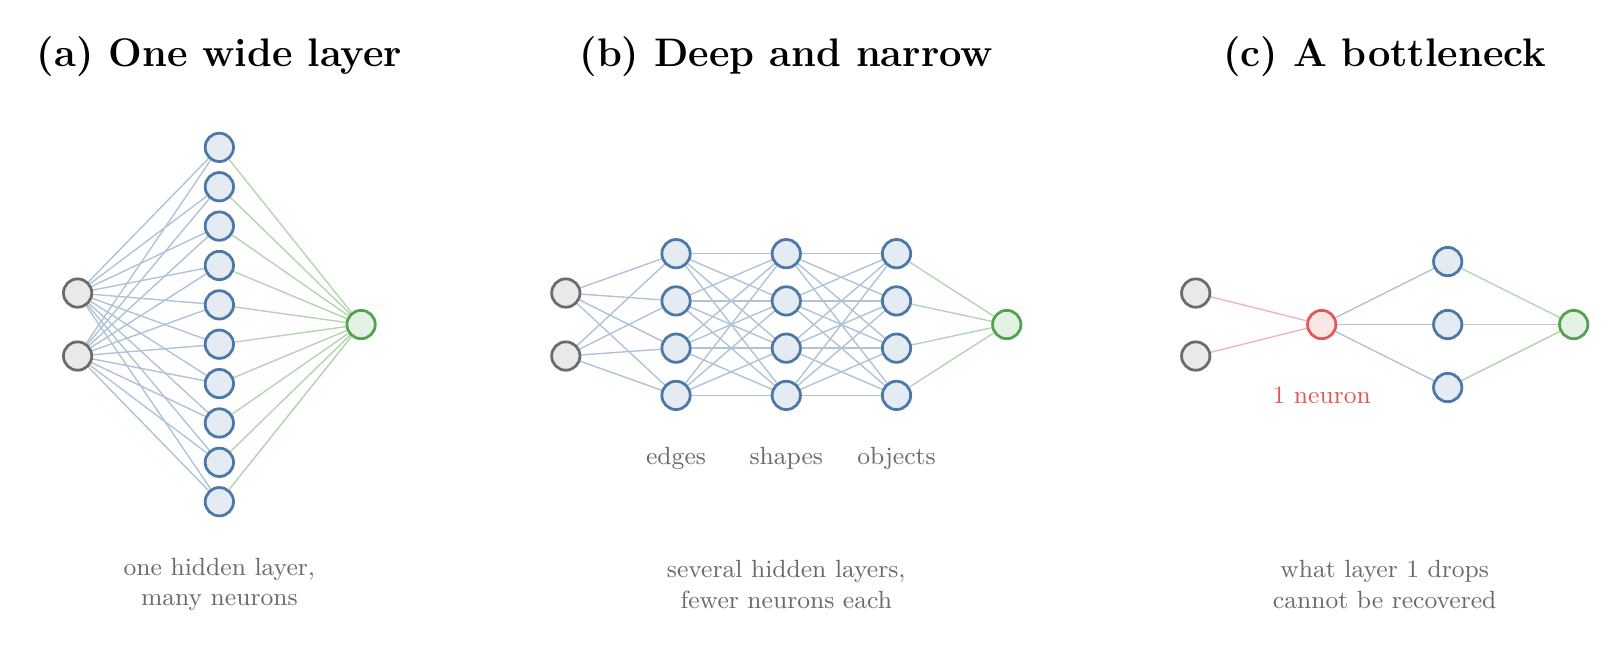
\begin{tikzpicture}[
  nd/.style={circle, draw=#1, fill=#1!15, minimum size=0.36cm, inner sep=0pt, line width=1pt},
  nd/.default=cblue]
  % helper: draw a column of n nodes centred at x, named <name>1..n
  \newcommand{\layer}[5]{% name, x, n, colour, spacing
    \foreach \k in {1,...,#3} \node[nd=#4] (#1\k) at (#2, {(\k - (#3+1)/2)*#5}) {};}
  \newcommand{\connect}[5]{% a, na, b, nb, colour
    \begin{scope}[on background layer]
      \foreach \i in {1,...,#2} \foreach \j in {1,...,#4} \draw[#5!45, line width=0.5pt] (#1\i) -- (#3\j);
    \end{scope}}
  % (a) one wide hidden layer
  \layer{a}{0}{2}{cgrey}{0.8}
  \layer{b}{1.8}{10}{cblue}{0.5}
  \layer{c}{3.6}{1}{cgreen}{0.8}
  \connect{a}{2}{b}{10}{cblue} \connect{b}{10}{c}{1}{cgreen}
  \node[title] at (1.8, 3.4) {(a) One wide layer};
  \node[note] at (1.8, -3.3) {one hidden layer,\\many neurons};
  % (b) three narrow hidden layers
  \begin{scope}[xshift=6.2cm]
    \layer{a}{0}{2}{cgrey}{0.8}
    \layer{b}{1.4}{4}{cblue}{0.6}
    \layer{d}{2.8}{4}{cblue}{0.6}
    \layer{e}{4.2}{4}{cblue}{0.6}
    \layer{c}{5.6}{1}{cgreen}{0.8}
    \connect{a}{2}{b}{4}{cblue} \connect{b}{4}{d}{4}{cblue} \connect{d}{4}{e}{4}{cblue} \connect{e}{4}{c}{1}{cgreen}
    \node[title] at (2.8, 3.4) {(b) Deep and narrow};
    \node[note] at (1.4, -1.7) {edges}; \node[note] at (2.8, -1.7) {shapes}; \node[note] at (4.2, -1.7) {objects};
    \node[note] at (2.8, -3.3) {several hidden layers,\\fewer neurons each};
  \end{scope}
  % (c) a bottleneck
  \begin{scope}[xshift=14.2cm]
    \layer{a}{0}{2}{cgrey}{0.8}
    \layer{b}{1.6}{1}{cred}{0.8}
    \layer{d}{3.2}{3}{cblue}{0.8}
    \layer{c}{4.8}{1}{cgreen}{0.8}
    \connect{a}{2}{b}{1}{cred} \connect{b}{1}{d}{3}{cblue} \connect{d}{3}{c}{1}{cgreen}
    \node[title] at (2.4, 3.4) {(c) A bottleneck};
    \node[note, text=cred] at (1.6, -0.9) {1 neuron};
    \node[note] at (2.4, -3.3) {what layer 1 drops\\cannot be recovered};
  \end{scope}
\end{tikzpicture}
\end{document}
